\documentclass[12pt]{article}
\usepackage[T1]{fontenc}
\usepackage[utf8]{inputenc}
\usepackage[russian]{babel}
\usepackage{amssymb,amsmath}
\usepackage{graphicx,color}
\usepackage{amsfonts}
\usepackage[colorlinks,urlcolor=blue]{hyperref}
\usepackage[ruled]{algorithm}
\usepackage[noend]{algorithmic}
\usepackage{hyperref}


%%%%%%%%%%%%%%%%%%%%%%%%%%%%%%%%%%%%%%%%%%%%%%%%%%%%%%%%%%%%%%%%%%%%%%%%%%%%%%%
% Оформление алгоритмов в пакетах algorithm, algorithmic
%%%%%%%%%%%%%%%%%%%%%%%%%%%%%%%%%%%%%%%%%%%%%%%%%%%%%%%%%%%%%%%%%%%%%%%%%%%%%%%

%Обнуление счетчика
\setcounter{algorithm}{0}

\textheight=24cm % высота текста
\textwidth=18cm % ширина текста
\oddsidemargin=-1cm % отступ от левого края
\topmargin=-3cm % отступ от верхнего края
\sloppy
\renewcommand{\baselinestretch}{1.1}
\renewcommand{\baselinestretch}{1.5}

%-- Обозначение вектора жирным символом
\def\vec#1{\mathchoice{\mbox{\boldmath$\displaystyle#1$}}
{\mbox{\boldmath$\textstyle#1$}} {\mbox{\boldmath$\scriptstyle#1$}} {\mbox{\boldmath$\scriptscriptstyle#1$}}}


\begin{document}
\thispagestyle{empty}

\begin{center}


\includegraphics[width=0.5\textwidth]{msu.eps}\\
{Московский государственный университет имени М.В.~Ломоносова}\\
Факультет вычислительной математики и кибернетики\\
Кафедра математических методов прогнозирования

\vspace{3cm}

{\Large Чабаненко~Владислав~Дмитриевич}

\vspace{1cm}

{\Large\bfseries Модификации метода стохастического градиентного спуска для задач машинного обучения с большими объемами данных
\\}

\vspace{1cm}

{\large ВЫПУСКНАЯ КВАЛИФИКАЦИОННАЯ РАБОТА}
\end{center}

\vfill

\begin{flushright}
  \textbf{Научный руководитель:}\\
  научный сотрудник\\
  Д.А.~Кропотов
\end{flushright}

\vfill

\begin{center}
Москва, 2016
\end{center}

\enlargethispage{3\baselineskip}

\newpage
\renewcommand{\contentsname}{Содержание}
\tableofcontents
\newpage

\section{Введение}


Нейронные сети способны решать широкий круг задач машинного обучения --- прогнозирование временных рядов \cite{time_series}, распознавание речи \cite{speech_recognition}, компьютерное зрение \cite{comp_vis} и т. д.

Актуальность проблемы обучения нейронных сетей в настоящее время связана с увеличением объемов данных, а так же архитектур сетей. В данной работе рассматривается \textit{метод стохастического градиентного спуска (SGD)} \cite{sgd} --- стандартный метод для обучения нейронных сетей, а так же его наиболее популярные модификации\footnote{\url{http://colinraffel.com/wiki/stochastic_optimization_techniques}}. Особое внимание в работе уделяется свежей разработке \cite{BN} для ускорения обучения нейронных сетей, называемой \textit{батч-нормализацией}. Мотивация нашего исследования состоит в том, что авторы обучали нейронную сеть с батч-нормализацией стандартным методом SGD, но не рассматривали его различные модификации. 

Цели работы: 
\begin{itemize}
\item исследовать применение батч-нормализации к различным модификациям метода SGD;
\item разработать рекомендации по использованию батч-нормализации.
\end{itemize}

Работа содержит два основных раздела: теоретический и экспериментальный. Теоретический раздел состоит из трех частей. Первая часть раскрывает суть искусственных нейронных сетей, описывает различные популярные архитектуры, кратко объясняет математическую модель нейронных сетей и способ их обучения. Во второй части описывается стандартный метод для обучения нейронных сетей --- метод стохастического градиентного спуска, и указывается его основной недостаток. Затем вводятся модификации стандартного метода, направленные на частичное устранение этого недостатка. Третья часть поднимает еще одну проблему, возникающую при обучении нейронных сетей, и описывает свежий подход по ее решению, называемый батч-нормализацией. Раздел, посвященный экспериментам, состоит из четырех частей. Первые две части описывают наборы данных и архитектуры нейронных сетей, используемые в работе. В третьей части подробно описываются постановки экспериментов и выдвигаемые гипотезы. Последняя часть содержит результаты экспериментов и выводы из них.


\section{Теоретическая часть}

\subsection{Нейронные сети в машинном обучении}


Искусственные нейронные сети в машинном обучении (artificial neural networks) --- это семейство моделей, созданных по подобию центральной нервной системы у животных. 

Они представляют собой систему связанных между собой нейронов, обменивающихся друг с другом сигналами (нервными импульсами). Для передачи сигнала служит синапс (место контакта между двумя нейронами). Синапсы хранят параметры нейронной сети, называемые весами, с помощью которых происходят манипуляции с сигналами.


Нейронные сети используются для аппроксимации функций, которые в общем случае неизвестны, и которые могут зависеть от большого количества признаков. С помощью нейронных сетей можно решать такие интересные и сложные задачи машинного обучения, как прогнозирование временных рядов, распознавание речи и компьютерное зрение.\\

Нейронная сеть может быть отображена как ориентированный граф. Первый слой нейронной сети называют \textit{входным слоем (input layer)}, последний --- \textit{выходным слоем (output layer)}. В общем случае нейронные сети могут иметь различную структуру слоев. Самая популярная архитектура --- многослойный персептрон (рис. \ref{fig:mlp}), в которой промежуточные слои называются \textit{скрытыми слоями (hidden layers)}. Благодаря наличию скрытых слоев нейронная сеть позволяет аппроксимировать очень сложные нелинейные функции.

\begin{figure}[h!]
\centering
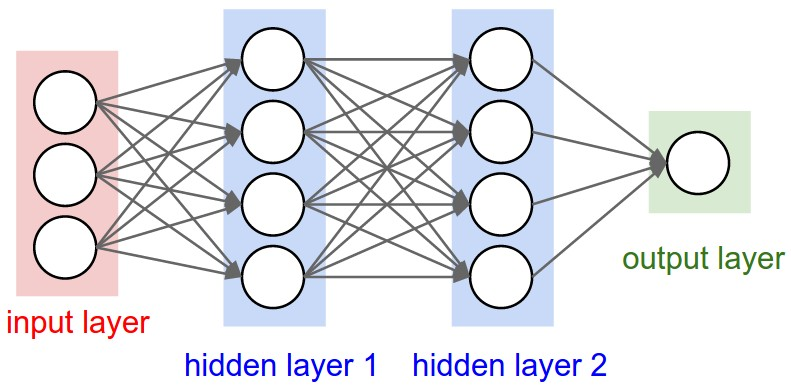
\includegraphics[scale=0.4]{mlp.jpeg}
\caption{Многослойный персептрон} \label{fig:mlp}
\end{figure}


Математически, функция нейронной сети $f(x)$ определяется как композиция функций $g_i(x)$, которые в свою очередь представляют композицию других функций. Широко распространенный тип композиции --- нелинейная взвешенная сумма $f(x) = \sigma(\sum_i w_i g_i(x))$, где $g_i$ --- активации нейронов с предыдущего слоя, $w_i$ --- веса линейной трансформации, а $\sigma$ --- некоторая заданная нелинейная функция активации. Наиболее часто используемые функции активации: \textit{сигмоида (sigmoid)}

\begin{equation}
\sigma(x) = \frac{1}{1 + \exp(-x)}
\end{equation}

или \textit{выпрямленный линейный элемент (rectified linear unit)}

\begin{equation}
\sigma(x) = max(x, 0).
\end{equation}


Нейронные сети по представлению графа разделяют на \textit{сети прямого распространения (feedforward)} и \textit{рекуррентные (recurrent)}. Первые представляют собой ациклический граф, вторые же, наоборот, соцержат циклы. Далее будут рассматриваться только сети прямого распространения.

Обычно, говоря про нейронные сети, подразумевают \textit{полносвязные} (как на рис. \ref{fig:mlp}), то есть когда в паре соседних слоев все нейроны связаны между собой. 

Однако есть и другие архитектуры сетей. Большой популярностью пользуются \textit{сверточные нейронные сети (convolutional neural networks)}. Эти нейронные сети специально спроектированы для работы с изображениями. Основная идея их применения --- автоматическое выделение признаков исходного изображения. Отличия сверточной нейронной сети от полносвязной состоят в наличии так называемых \textit{сверточных слоёв (convolutional layers)}, а также \textit{слоёв, уменьшающих размерность (subsampling layers)}. 

Свёрточный слой принимает на вход изображение $X$, а затем применяет к каждому окну изображения, фиксированного размера, свертку с ядром $W$, то есть преобразует каждый фрагмент исходного изображения в один новый пиксель $Y$ (рис. \ref{fig:conv1}, \ref{fig:conv2}).


\begin{figure}[h!]
\centering
\begin{minipage}{0.49\linewidth}
\centering
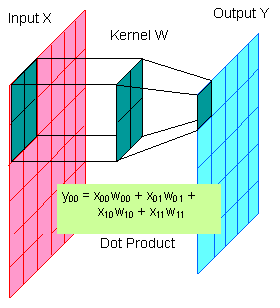
\includegraphics[scale=0.6]{conv1.png}
\caption{Первый пиксель}\label{fig:conv1}
\end{minipage} \hfill
\begin{minipage}{0.49\linewidth}
\centering
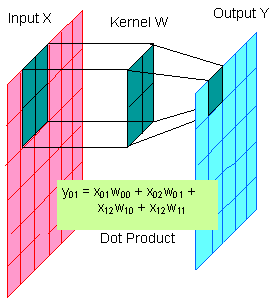
\includegraphics[scale=0.6]{conv2.png}
\caption{Второй пиксель}\label{fig:conv2}
\end{minipage}
\end{figure}


Таким образом, полученное изображение на выходе будет меньшего размера, и каждый нейрон на выходе будет связан лишь с некоторыми близлежащими нейронами входа (только с теми нейронами, которые участвуют в свертке). 

Если к изображению будет применяться свертка только одним ядром, то сеть научится выделять только один вид признаков. Поэтому обычно сверточный слой состоит из нескольких изображений одинакового размера --- \textit{карт признаков (feature maps)}. Различаются карты только значениями параметров (весами свертки). 

Другой вид слоев \textit{(subsampling layers)} используется для того, чтобы нейронная сеть была инвариантной к некоторым простым преобразованиям исходной картинки (небольшим сдвигам или искажениям). Простейший пример такого слоя: \textit{макс-пулинг (max-pooling)}. В этом слое мы проходим по непересекающимся окнам $k \times k$ изображения и на выход посылаем только максимум из рассматриваемых значений. Таким образом, полученное изображение на выходе будет иметь ширину и высоту в $k$ раз меньше. 

Обычно для получения признаков более высокого порядка применяют многократно эти два слоя. Также в конце сети обычно помещают полносвязный слой, который будет принимать на вход полученные признаки и проводить классификацию изображения.\\

Рассмотрим вопрос обучения нейронных сетей. По данной задаче и классу функций $F$ обучение означает использование множества наблюдений для нахождения функции $f^* \in F$, которая решает задачу в некотором оптимальном смысле.

Для определения оптимального решения вводится функционал эмпирического риска (например, как в \eqref{eq:empirical_risk}) $C: F \rightarrow \mathbb{R}$ такой, что $f^*: C(f^*) \leq C(f) \ \forall f \in F,$ то есть нет других решений, для которых функция риска была бы меньше, чем для оптимального решения.

Когда решение зависит от данных, функция эмпирического риска должна быть функцией от наблюдаемых данных, иначе не будет возможности смоделировать ничего, соответствующего данным. Одна из классических задач машинного обучения --- задача обучения с учителем: у нас есть набор данных $X$ и ответы на данных $Y$, требуется настроить параметры модели, чтобы как можно лучше описать наблюдаемые данные. Один из способов настройки нейронной сети на такую задачу: минимизировать отклонение предсказанных ответов на данных от реальных ответов, используя, например, среднеквадратичную функцию эмпирического риска: 
\begin{equation}\label{eq:empirical_risk}
\begin{aligned}
\hat{C}(f) =\frac{1}{N}\sum_{i=1}^N \left( f(x_i, \theta)-y_i \right) ^2,
\end{aligned}
\end{equation}

где оптимизация ведется по параметрам $\theta$, если вид функции $f$ зафиксирован.\\


Стандартный алгоритм для обучения нерйонных сетей --- \textit{алгоритм обратного распространений ошибки (backpropagation)} \cite{backprop}. Вообще говоря, это метод для подсчета градиента по нейронной сети: от последнего слоя к первому поочередно вычисляется градиент функции риска по параметрам текущего слоя. Такое вычисление возможно благодаря тому, что нейронная сеть представляет собой композицию функций, и для нее можно использовать правило дифференцирования сложной функции\footnote{\url{https://en.wikipedia.org/w/index.php?title=Chain_rule&oldid=717805710}}.


\subsection{Метод стохастического градиентного спуска и его модификации}

Нейронные сети часто обучаются стохастически, то есть на разных итерациях используются разные части данных. Это мотивировано, как минимум, двумя причинами: во-первых, наборы данных, используемые для обучения, часто очень большие, чтобы хранить их полностью в оперативной памяти и/или производить вычисления эффективно; во-вторых, оптимизируемая функция обычно невыпуклая, таким образом, использование разных частей данных на каждой итерации может помочь от застревания модели в локальном минимуме. Кроме того, обучение нейронных сетей обычно производится с помощью градиентных методов первого порядка, так как из-за большого количества параметров в нейронной сети невозможно эффективно применять методы более высоких порядков.

Стандартным методом обучения нейронных сетей является метод стохастического градиентного спуска (SGD). Однако он может расходиться или сходиться очень медленно, если шаг обучения настроен недостаточно аккуратно. Поэтому существует много альтернативных методов с целью ускорить сходимость обучения и избавить пользователя от необходимости тщательной настройки гиперпараметров. Эти методы часто более эффективно вычисляют градиенты и адаптивно изменяют шаг обучения по итерациям. Рассмотрим подробнее метод SGD и несколько его наиболее популярных модификаций.


\paragraph{Стохастический градиентный спуск (SGD) \cite{sgd}} обновляет каждый параметр, вычитая градиент оптимизируемой функции по соответствующему параметру и масштабируя его на \textit{шаг обучения} $\eta$, являющийся гиперпараметром. Если $\eta$ слишком большой, то метод будет расходиться; если слишком маленький --- будет сходиться медленно. Правило пересчета:


\begin{equation}
\begin{aligned}
i &\sim \mathcal{U}\{1, 2, \ldots, n\}\\
\theta_{t+1} &= \theta_t - \eta \nabla f_i(\theta_t),
\end{aligned}
\end{equation}

где $f_i$ --- функция, подсчитанная на $i$-ом \textit{мини-батче} (части) данных, и индекс $i$ выбирается случайным образом.

\paragraph{Стохастический градиентный спуск с инерцией (SGDm) \cite{momentum}\\}

В методе SGD градиент $\nabla f_i(\theta_t)$ часто быстро изменяется на каждой итерации, так как функционал вычисляется на разных данных. Это изменение частично смягчается, если использовать градиенты с прошлых итераций, масштабированные на некоторый \textit{гиперпараметр инерции} $\mu$ по следующей формуле \textit{(идея инерции)}:


\begin{equation}
\begin{aligned}
v_{t+1} &= \mu v_t - \eta \nabla f_i(\theta_t)\\
\theta_{t+1} &= \theta_t + v_{t+1}
\end{aligned}
\end{equation}

%Утверждается, что добавление градиентов с предыдущих итераций имеет эффект аппроксимации некоторой информации второго порядка о градиенте.

\paragraph{Метод адаптивного градиента (Adagrad) \cite{adagrad}} эффективно перемасштабирует шаг обучения для каждого параметра в отдельности, учитывая историю всех прошлых градиентов для этого параметра \textit{(идея масштабирования)}. Это делается путем деления каждого элемента в градиенте $\nabla f_i$ на квадратный корень суммы квадратов прошлых соответствующих элементов градиента. Перемасштабирование таким способом эффективно уменьшает шаг обучения для параметров, которые имеют большую величину градиента. Также метод уменьшает сам шаг обучения со временем, так как сумма квадратов увеличивается с каждой итерацией. При инициализации масштабирующего параметра $g = 0$ формула для пересчета имеет вид

\begin{equation}
\begin{aligned}
g_{t+1} &= g_t + \nabla f_i(\theta_t) ^2\\
\theta_{t+1} &= \theta_t - \frac{\eta \nabla f_i(\theta_t)}{\sqrt{g_{t+1} + \epsilon}},
\end{aligned}
\end{equation}

где деление выполняется поэлементно, а $\epsilon$ --- это небольшая константа, введенная для численной стабильности. Метод имеет хорошие теоретические гарантии и практические результаты~\cite{adagrad}

\paragraph{Метод адаптивного скользящего среднего градиентов (RMSprop)} \cite{rmsprop} очень похож по принципу работы на метод Adagrad. Единственное его отличие в том, что шкалирующий член $g_t$ вычисляется, как экспоненциальное скользящее среднее вместо кумулятивной суммы. Это делает $g_t$ оценкой второго момента градиента $\nabla f$ и устраняет тот факт, что шаг обучения со временем уменьшается. Правило пересчета:

\begin{equation}
\begin{aligned}
g_{t+1} &= \gamma g_t + (1 - \gamma) \nabla f_i(\theta_t)^2\\
\theta_{t+1} &= \theta_t - \frac{\eta \nabla f_i(\theta_t)}{\sqrt{g_{t+1} + \epsilon}}
\end{aligned}
\end{equation}


%In the original lecture slides where it was proposed, γ is set to .9. In 8), it is shown that the gt+1−−−√ term approximates (in expectation) the diagonal of the absolute value of the Hessian matrix (assuming the update steps are N(0,1) distributed). It is also argued that the absolute value of the Hessian is better to use for non-convex problems which may have many saddle points. 

\paragraph{Метод адаптивного шага обучения (Adadelta)} \cite{adadelta} использует аналогичное экспоненциальное скользящее среднее для оценки второго момента градиента $g_t$, как и RMSprop. Также метод вычисляет скользящее среднее $x_t$ по $v_t$, аналогичным инерции, но при обновлении этой величины, используется квадрат текущего шага. Обновление параметров происходит по следующим формулам:

%Adadelta 10) uses the same exponentially decaying moving average estimate of the gradient second moment gt as RMSProp. It also computes a moving average xt of the updates vt similar to momentum, but when updating this quantity it squares the current step, which I don't have any intuition for. 

\begin{equation}
\begin{aligned}
g_{t+1} &= \gamma g_t + (1 - \gamma) \nabla f_i(\theta_t)^2\\
v_{t+1} &= - \frac{\sqrt{x_t + \epsilon} \nabla f_i(\theta_t)}{\sqrt{g_{t+1} + \epsilon}}\\
x_{t+1} &= \gamma x_t + (1 - \gamma) v_{t+1}^2\\
\theta_{t+1} &= \theta_t + v_{t+1}
\end{aligned}
\end{equation}

\begin{figure}[h!]
\centering
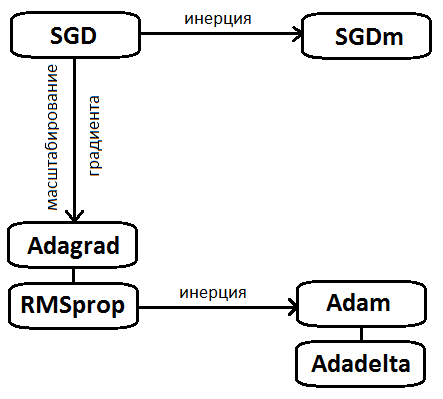
\includegraphics[scale=0.6]{methods.png}
\caption{Интуиция и связь модификаций метода SGD} \label{intuition}
\end{figure}

\newpage
\paragraph{Метод адаптивной инерции (Adam) \cite{adam}} похож на каждый из трех предыдущих методов (Adagrad, Adadelta, RMSprop). Отличается он от них двумя идеями: во-первых, оценка первого момента вычисляется как скользящее среднее; во-вторых, из-за того, что оценки первого и второго моментов инициализируются нулями, используюется небольшая коррекция, чтобы результирующие оценки не были смещены к нулю. Метод также инвариантен к масштабированию градиентов. При заданных гиперпараметрах $\gamma_1, \gamma_2, \lambda, \eta$ и $m_0 = 0, g_0 = 0$ правило пересчета следующее: \cite{adam}

\begin{equation}
\begin{aligned}
m_{t+1} &= \gamma_1 m_t + (1 - \gamma_1) \nabla f_i(\theta_t)\\
g_{t+1} &= \gamma_2 g_t + (1 - \gamma_2) \nabla f_i(\theta_t)^2\\
\hat{m}_{t+1} &= \frac{m_{t+1}}{1 - \gamma_1^{t+1}}\\
\hat{g}_{t+1} &= \frac{m_{t+1}}{1 - \gamma_2^{t+1}}\\
\theta_{t+1} &= \theta_t - \frac{\eta \hat{m}_{t+1}}{\sqrt{\hat{g}_{t+1} + \epsilon}}
\end{aligned}
\end{equation}

На рис. \ref{intuition} отображена связь всех рассмотренных методов. Таким образом, каждый метод использует либо идею \textit{масштабирования градиента} (Adagrad, RMSprop),\ либо идею \textit{инерции} (SGDm),\ либо сразу обе идеи (Adam и Adadelta).



\subsection{Батч-нормализация}

Помимо настройки шага для обучения нейронной сети возникает еще одна неочевидная на первый взгляд проблема. Когда обучающей системе на вход подаются данные, имеющие разную природу (например, распределение на данные изменяется со временем), система замедляется в обучении, так как ей приходится долго адаптироваться под изменяющиеся условия. В литературе такой эффект носит название \textit{ковариационного сдвига (covariate shift)} \cite{cov_shift}. В случае нейронных сетей такая проблема возникает на внутренних слоях. Представим, что каждый слой нейронной сети --- это отдельная компонента обучающей системы. Тогда каждый слой (кроме самого первого) получает на вход данные, полученные с выхода предыдущего слоя. А так как в процессе обучения параметры сети меняются, то и распределение на данные, подаваемые на вход внутренних слоев, тоже меняется. Особенно сильно такой эффект наблюдается на более глубоких слоях. Так, даже небольшие изменения на входе нейронной сети сильно влияют на последующие слои --- меняется распределение на нейроны, входящие во внутренние слои сети.

Установлено \cite{eff_backprop}, что обучение сходится быстрее, если предварительно \textit{нормализовать} (сделать нулевое матожидание и единичные диспресии) и \textit{декоррелировать} входные данные для компоненты обучающей системы. Тогда для нейронной сети хотелось бы нормализовать данные перед входом на каждый слой. Таким образом и действует метод \textit{батч-нормализации (batch normalization)}, предложенный в 2015 году \cite{BN}.

Рассмотрим подробнее структуру батч-нормализации на примере одного внутреннего слоя.

\begin{itemize}

\item Пусть нормализуемы слой имеет размерность $d$: $x = (x_1, \ldots, x_d)$. Тогда можно нормализовать $k$-ое измерение $x$ по следующей формуле (для простоты все измерения нормализуются независимо):

\begin{equation}\label{eq:normalization}
\hat{x}^k = \frac{x^k - \mathbb{E}[x^k]}{\sqrt{\mathrm{Var}[x^k]}}
\end{equation}

Мы также должны масштабировать и сдвинуть нормализованную величину. В противном случае, лишь нормализация ограничит репрезентативную способность слоя. Например, если нормализуется вход на сигмоиду, то на выходе будет наблюдаться близкое к линейному преобразование (так как сигмоида $\sigma(x) = \frac{1}{1 + \exp(-x)}$ на отрезке $[-1, 1]$ похожа на линейную функцию).

\item Таким образом, нормализованная величина трансформируется в новую:

\begin{equation}
y^k = \gamma^k \hat{x}^k + \beta^k,
\end{equation}

где параметры $\gamma, \beta$ настраиваются в процессе обучения для каждой размерности.

\item 
Более того, как в стохастическом градиентном спуске используются мини-батчи, можно так же использовать их в нормализации для оценки матожидания и дисперсии для каждого нейрона
\begin{equation}
\begin{aligned}
\mu_B &= \frac{1}{m} \sum_{i=1}^m x^k_i, \\
\sigma_B^2 &= \frac{1}{m} \sum_{i=1}^m (x^k_i - \mu_B)^2,
\end{aligned}
\end{equation}
где $B = \{x^k_{1, \ldots, m}\}$ --- текущий мини-батч для $k$-го нейрона. Тогда вместо $\mathbb{E}[x^k]$ и $\mathrm{Var}[x^k]$ в \eqref{eq:normalization} можно подставить значения $\mu_B$ и $\sigma_B^2$, являющиеся оценками соответствующих величин по мини-батчу.

\item Итоговое преобразование добавляется в нейронную сеть перед нелинейной функцией активации.
\end{itemize}


В итоге батч-нормализация

\begin{itemize}
\item уменьшает ковариационный сдвиг во внутренних слоях нейронной сети и следовательно ускоряет обучение;
\item является дифференцируемым преобразованием, то есть для обучения сети все так же можно применять метод обратного распространения ошибки;
\item позволяет использовать большие шаги обучения, то есть позволяет не слишком аккуратно настраивать гиперпараметр шага;
\item не производит явную декорреляцию входных данных для различных нейронов одного слоя.
\end{itemize}


В оригинальной статье \cite{BN} нейронная сеть с батч-нормализацией обучалась с помощью обычного метода SGD. В данной работе исследуется сочетание батч-нормализации и рассмотренных выше модификаций метода SGD.


\section{Эксперименты}

\subsection{Наборы данных} \label{datasets}

В рамках работы исследования проводились для задачи многоклассовой классификации на следующих наборах данных:

\begin{itemize}
\item MNIST\footnote{\url{http://yann.lecun.com/exdb/mnist}}, рис. \ref{fig:mnist} (70 тыс. рукописных цифр --- 10 классов): выборка была поделена на тренировочную (50 тыс.), валидационную (10 тыс.) и тестовую (10 тыс.)
 
\item CIFAR-10\footnote{\url{https://www.cs.toronto.edu/~kriz/cifar.html}}, рис. \ref{fig:cifar10} (60 тыс. изображений --- 10 классов): выборка поделена на тренировочную (40 тыс.), валидационную (10 тыс.) и тестовую (10 тыс.)
\end{itemize}

\begin{figure}[h!]
\centering
\begin{minipage}{0.45\linewidth}
\centering
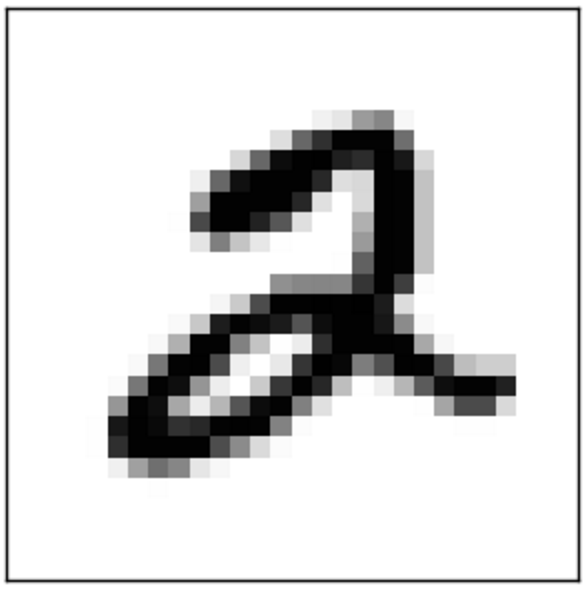
\includegraphics[scale=0.3]{mnist_img.png}
\caption{Пример объекта из набора данных MNIST} \label{fig:mnist}
\end{minipage} \hfill
\begin{minipage}{0.45\linewidth}
\centering
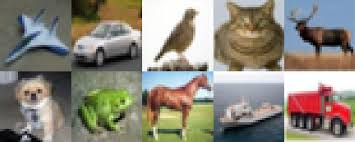
\includegraphics[scale=0.6]{cifar_img.jpeg}
\caption{Примеры изображений из набора данных CIFAR-10} \label{fig:cifar10}
\end{minipage}
\end{figure}

\subsection{Архитектуры нейронных сетей} \label{arch}

Для дальнейших экспериментов были выбраны конкретные архитектуры сетей. Опишем четыре варианта сети, над которыми проводились эксперименты:

\begin{itemize}
\item полносвязная сеть (multilayer perceptron, MLP): состоит из 3-х скрытых слоёв по 100 нейронов;
\item сверточная сеть (convolutional neural network, CNN): состоит из 2-х сверточных слоёв (32 карты признаков со сверткой $5 \times 5$ + слой max-pooling с размером окна $2 \times 2$), затем один полносвязный слой с 256 нейронами;
\item полносвязная глубокая сеть (deep MLP): состоит из 20-ти скрытых слоёв по 30 нейронов;
\item сверточная глубокая сеть (deep CNN): состоит из 5-ти идущих подряд сверточных подсетей (3 сверточных слоя ($k$ карт признаков с сверткой $3 \times 3$ + max-pooling с размером окна $2 \times 2$)), где для каждой следующей подсети $k$ увеличивается в два раза: $[32, 64, 128, 256, 512]$, а затем следует один полносвязный слой с 256 нейронами;
\end{itemize}

В полносвязную сеть батч-нормализация добавляется сразу после линейной трансформации и перед функцией активации. Для сверточной сети --- сразу после свертки и перед активацией.

В качестве функции активации во всех архитектурах используется выпрямленный линейный элемент (ReLU). Также на выходе каждой сети есть еще один полносвязный слой с выходом на $10$ нейронов с многопеременной логистической функцией активации (softmax)\footnote{\url{http://ufldl.stanford.edu/tutorial/supervised/SoftmaxRegression/}}.


\subsection{Постановки экспериментов}

В данном разделе исследуется, как влияет добавление батч-нормализации на различные модификации метода стохастического градиентного спуска при обучении нейронных сетей.\\

Перед тем, как приступить к экспериментам, сформулируем несколько гипотез:
\begin{itemize}
\item добавление батч-нормализации в сеть увеличивает скорость сходимости обучения сети для всех методов;
\item чем метод сложнее, тем батч-нормализация слабее ускоряет его сходимость;
\item батч-нормализация сильнее проявляет ускорение обучения на глубоких сетях.
\end{itemize}

\newpage
\paragraph{Влияние батч-нормализации на все методы.\\}

В первом эксперименте оценивается, на сколько изменяется качество обучения методов при добавлении батч-нормализации. Для этого выполняются следующие пункты: 

\begin{enumerate}
\item Выбираются исследуемые методы: SGD, SGDm, Adam, Adagrad, Adadelta, RMSprop.
\item Выбираются наборы данных: MNIST, CIFAR-10 (описаны в \ref{datasets}).
\item Выбираются архитектуры сети: MLP и CNN (описаны в \ref{arch}).
\item Для всех исследуемых методов подюирается оптимальный шаг обучения (по качеству на тестовой выборке) на всех комбинациях рассматриваемых архитектур и наборов данных. Для этого сначала грубо оценивается приемлемый порядок шага обучения с помощью перебора значений по сетке. Затем в окрестности полученной величины перебирается значение шага по более частой сетке. В результате выбирается лучший шаг обучения из рассмотренных.
\item Сохраняются полученные результаты работы всех методов на тренировочных и валидационных выборках по эпохам, а также результаты на тестовых выборках.
\item Составляются таблицы относительных улучшений качества всех методов при добавлении в сеть батч-нормализации на тестовых выборках для всех пар наборов данных и архитектур.
\item Исследуются полученные результаты на наличие закономерностей.
\end{enumerate}


\paragraph{Влияние батч-нормализации на методы при обучении глубоких нейронных сетей.\\}

Во втором эксперименте проверяется, что изменится для всех методов на глубоких сетях. Для этого выполняются следующие пункты:

\begin{enumerate}
\item Выбираются исследуемые методы из предыдущего эксперимента: SGD, SGDm, Adam, Adagrad, Adadelta, RMSprop.
\item Выбираются наборы данных из предыдущего эксперимента: MNIST, CIFAR-10.
\item Выбираются архитектуры для глубокой сети: deep MLP, deep CNN (описаны в \ref{arch}).
\item Для всех исследуемых методов подбирается оптимальный шаг обучения на всех комбинациях рассматриваемых глубоких архитектур и датасетов аналогично предыдущему эксперименту.
\item Сохраняются полученные результаты работы всех методов на тренировочных и валидационных выборках по эпохам, а также результаты на тестовых выборках.
\item Составляются таблицы относительных улучшений качества всех методов при добавлении в глубокую сеть батч-нормализации на тестовых выборках для всех пар датасетов и архитектур.
\item Сравниваются результаты с соответствующими результатами из предыдущего эксперимента.
\end{enumerate}

Для вычисления \textit{относительного улучшения} качества используется следующая формула:

\begin{equation}
\mathrm{rel} = \frac{y - x}{100 - x},
\end{equation}

где $x$ --- качество метода (в процентах) до добавления батч-нормализации, $y$ --- качество после добавления батч-нормализации (заметим, что всегда $\mathrm{rel} \leq 1$). Величина $\mathrm{rel}$ показывает, например, что улучшение с $50 \%$ до $51 \%$ менее значимо, чем улучшение с $90 \%$ до $91 \%$.

%\paragraph{Исследование работы метода Adam при добавлении в сеть батч-нормализации.}
%
%В ходе экспериментов неоднократно наблюдалось, что после добавления в сеть батч-нормализации метод Adam начинал при обучении совершать непредсказуемые скачки по качеству как на валидационной, так и на тренировочной выборках. 

%\begin{enumerate}
%\item Выберем простой датасет: MNIST
%\item Выберем архитектуры сети: MLP, CNN (неглубокие)
%\item Добавим в исходники сохранение $v_t$ по итерациям (скользящее среднее квадратов градиентов)
%\item Запустим БН Адам несколько раз при стандартных параметрах -- убедимся в наличии скачков, посмотрим, как себя ведут $v_t$ в эти моменты
%\item Запустим Адам при стандартных параметрах
%\item Запустим БН Адам несколько раз при $\epsilon = 10^{-4}$ и $\epsilon = 10^{-2}$ -- убедимся, что скачки стали меньше, и что $v_t$ стали больше
%\item Проверим, как влияет на качество увеличение $\epsilon$ и сравним все со стандартным методом Адам
%\end{enumerate}


\subsection{Результаты экспериментов}

\paragraph{Влияние батч-нормализации на все методы.\\}

Из таблицы~\ref{table:1} видно, что все относительные улучшения положительны. Однако для методов SGDm, Adam и Adadelta для архитектуры MLP наблюдается очень слабое улучшение.  Как обнаружится далее, качество этих методов может и понижаться на некоторых эпохах при добавлении в сеть батч-нормализации. Также отметим, что сильнее всего батч-нормализация улучшает качество метода SGD, как самого простого метода.

\begin{table}[h!]
\centering
\begin{tabular}{|c|c|c|c|c|c|c|c|}\hline
\textbf{Методы} & \textbf{MNIST + MLP} & \textbf{CIFAR-10 + MLP} & \textbf{MNIST + CNN} & \textbf{CIFAR-10 + CNN} \\\hline
\textbf{SGD} & \textbf{0.24} & \textbf{0.2} & \textbf{0.35} & \textbf{0.36} \\\hline
SGDm & 0.06 & 0.1 & 0.29 & 0.25 \\\hline
Adam & 0.05 & 0.09 & 0.13 & 0.14 \\\hline
Adagrad & 0.13 & 0.17 & 0.3 & 0.33 \\\hline
Adadelta & 0.03 & 0.11 & 0.19 & 0.2 \\\hline
RMSprop & 0.22 & 0.16 & 0.24 & 0.19 \\\hline
\end{tabular}
\caption{Улучшение качества на тестовой выборке при добавлении батч-нормализации} \label{table:1}
\end{table}

Попробуем выявить закономерности в полученных результатах. Посмотрим отдельно на результаты для архитектуры CNN для датасетов MNIST (табл. \ref{table:2.mnist}) и CIFAR-10 (табл. \ref{table:2.cifar}).


\begin{table}[h!]
\centering
\small
\begin{minipage}{0.45\linewidth}
\centering
\begin{tabular}{|c|c|c|c|c|c|c|c|c|c|}\hline
\textbf{Номер эпохи} & \textbf{2} & \textbf{5}  & \textbf{20}  & \textbf{35} & \textbf{50} \\\hline

SGD & 0.64 & 0.57  & 0.48  & 0.49 & 0.37 \\\hline

SGDm & 0.7 & 0.52  & 0.47  & 0.34 & 0.3 \\\hline

\textbf{Adam} & \textbf{0.44} & \textbf{0.17}  & \textbf{0.29}  & \textbf{0.15} & \textbf{0.11} \\\hline

Adagrad & 0.46 & 0.38  & 0.31 & \textbf{0.3} & 0.33 \\\hline

\textbf{Adadelta} & \textbf{0.19} & \textbf{0.07}  & \textbf{0.23} & \textbf{0.15} & \textbf{0.18} \\\hline

\textbf{RMSprop} & \textbf{0.34} & \textbf{0.22}  & \textbf{0.11}  & 0.36 & \textbf{0.27} \\\hline
\end{tabular}
\caption{\small Улучшения качества при добавлении батч-нормализации в сеть CNN, MNIST. \textbf{Жирным} выделены топ-3 наименьшего улучшения (по столбцам)} \label{table:2.mnist}
\end{minipage} \hfill
\begin{minipage}{0.45\linewidth}
\centering
\begin{tabular}{|c|c|c|c|c|c|}\hline
\textbf{Номер эпохи} & \textbf{2} & \textbf{5} & \textbf{20} & \textbf{35} & \textbf{50} \\\hline
SGD & 0.32 & 0.4 & 0.3 & 0.34 & 0.32 \\\hline

SGDm & 0.34 & 0.34 & 0.35 & 0.27 & 0.24 \\\hline

\textbf{Adam} & \textbf{0.19} & \textbf{0.22} & \textbf{0.23} &\textbf{ 0.2} & \textbf{0.15} \\\hline

Adagrad & \textbf{0.26} & \textbf{0.26} & 0.35 & 0.37 & 0.35 \\\hline

\textbf{Adadelta} & 0.27 & 0.34 & \textbf{0.17} & \textbf{0.22} & \textbf{0.22} \\\hline

\textbf{RMSprop} & \textbf{0.23} & \textbf{0.22} & \textbf{0.26} & \textbf{0.21} & \textbf{0.19} \\\hline

\end{tabular}
\caption{\small Улучшения качества при добавлении батч-нормализации в сеть CNN, CIFAR-10. \textbf{Жирным} выделены топ-3 наименьшего улучшения (по столбцам)} \label{table:2.cifar}
\end{minipage} 
\end{table}


В таблицах показаны улучшения для валидационных выборок. Здесь можно обнаружить следующую закономерность: слабее всего улучшаются методы Adam, Adadelta и RMSprop, которые используют для оценки второго момента градиента экспоненциальное скользящее среднее (методы, наследуемые от RMSprop на рис.\ref{intuition}).\\


Теперь посмотрим на такие же результаты для архитектуры MLP для датасетов MNIST (табл. \ref{table:3.mnist}) и CIFAR-10 (табл. \ref{table:3.cifar}).

\begin{table}[h!]
\centering
\small
\begin{minipage}{0.45\linewidth}
\centering
\begin{tabular}{|c|c|c|c|c|c|}\hline
\textbf{Номер эпохи} & \textbf{2} & \textbf{5} & \textbf{10} & \textbf{25} & \textbf{50} \\\hline
SGD & 0.67 & 0.63 & 0.42 & 0.25 & 0.22 \\\hline

\textbf{SGDm} & 0.47 & 0.34 &  \textbf{0.13} &  \color{red}\textbf{-0.08} &  \textbf{0.05} \\\hline

\textbf{Adam} &  \textbf{0.21} &  \textbf{0.2} & \color{red}\textbf{-0.05} & \color{red}\textbf{-0.15} & \textbf{0.07} \\\hline

Adagrad & 0.34 & 0.27 & 0.17 & 0.12 & 0.14 \\\hline

\textbf{Adadelta} & \textbf{0.3} & \textbf{0.08} & \textbf{0.08} & \color{red}\textbf{-0.0} & \textbf{0.03} \\\hline

RMSprop & \textbf{0.28} & \textbf{0.27} & 0.35 & 0.21 & 0.25 \\\hline

\end{tabular}
\caption{\small Улучшения качества при добавлении батч-нормализации в сеть MLP, MNIST. \textbf{Жирным} выделены топ-3 наименьшего улучшения (по столбцам)} \label{table:3.mnist}
\end{minipage} \hfill
\begin{minipage}{0.45\linewidth}
\centering
\begin{tabular}{|c|c|c|c|c|c|c|}\hline
\textbf{Номер эпохи} & \textbf{2} & \textbf{5} & \textbf{10} & \textbf{25} & \textbf{50} \\\hline

SGD & 0.23 & 0.18 & 0.22 & 0.21 & 0.17 \\\hline

\textbf{SGDm} & \textbf{0.17} & \textbf{0.13} & \textbf{0.15} & \textbf{0.13} & \textbf{0.1} \\\hline

\textbf{Adam} & \textbf{0.13} &\textbf{ 0.12} & \textbf{0.11} & \textbf{0.1}3 & \textbf{0.12} \\\hline

Adagrad & 0.25 & 0.23 & 0.23 & 0.18 & 0.17 \\\hline

\textbf{Adadelta} & \textbf{0.18} & \textbf{0.14} & \textbf{0.19} & \textbf{0.17} & \textbf{0.15} \\\hline

RMSprop & 0.2 & 0.18 & 0.21 & 0.22 & 0.16 \\\hline

\end{tabular}
\caption{\small Улучшения качества при добавлении батч-нормализации в сеть MLP, CIFAR-10. \textbf{Жирным} выделены топ-3 наименьшего улучшения (по столбцам)} \label{table:3.cifar}
\end{minipage}
\end{table}


Первое, что бросается в глаза, так это отрицательная величина изменения качества (выделены \color{red}{\textbf{жирным красным}}\color{black}). Можно сделать вывод, что батч-нормализация не всегда повышает качество на промежуточных эпохах.\\

В таблицах \ref{table:3.mnist} и \ref{table:3.cifar} также указаны улучшения для валидационных выборок. Здесь наблюдаются следующие закономерности: слабее всего улучшаются методы SGDm, Adam и Adadelta, которые используют идею инерции (рис.\ref{intuition}). Также отметим, что результаты для одинаковых архитектур получаются похожими.

Из полученных результатов можно сделать вывод, что, чем идейно сложнее методы, тем они слабее улучшаются при добавлении батч-нормализации. Так, методы Adam и Adadelta в схеме \ref{intuition}  используют идеи масштабирования градиента и инерции --- и как раз для них батч-нормализация дает наименьшую прибавку.\\


Возникает идея, что добавление батч-нормализации в нейронную сеть слабее улучшает методы, которые и так показывают лучшее качество. Покажем, что это не совсем так.

Из таблицы \ref{table:5} хорошо видно, что метод SGDm показывает довольно высокое качество, однако не входит в топ-3 методов, для которых батч-нормализация дает наименьшее улучшение.

%\begin{table}
%\centering
%\begin{tabular}{|c|c|c|c|c|c|c|c|c|c|}\hline
%Номер эпохи & 2 & 5 & 8 & 15 & 20 & 35 & 50 \\\hline\hline
%
%SGD & 96.37 & 97.71 & 98.14 & 98.49 & 98.51 & 98.46 & 98.8 \\\hline
%
%SGDm & 95.89 & 97.75 & 98.12 & 98.42 & 98.43 & 98.77 & 98.82 \\\hline
%
%\textbf{Adam} & 97.64 & 98.57 & \color{green}\textbf{98.81} & \color{green}\textbf{98.92} & \color{green}\textbf{99.08} & \color{green}\textbf{99.12} & \color{green}\textbf{99.16} \\\hline
%
%Adagrad & \color{green}\textbf{98.0} & \color{green}\textbf{98.}6 & \color{green}\textbf{98.81} & 98.91 & \color{green}\textbf{99.01} & 98.92 & 98.96 \\\hline
%
%\textbf{Adadelta} & \color{green}\textbf{98.16} & \color{green}\textbf{98.61} & \color{green}\textbf{98.95} & \color{green}\textbf{99.1} & \color{green}\textbf{99.11} & \color{green}\textbf{99.22} & \color{green}\textbf{99.22} \\\hline
%
%\textbf{RMSprop} & \color{green}\textbf{97.87} & \color{green}\textbf{98.73} & \color{green}\textbf{98.92} &\color{green}\textbf{ 99.1} & 98.91 & \color{green}\textbf{98.97} & \color{green}\textbf{99.1} \\\hline
%
%\end{tabular}
%\caption{Качество на MNIST, CNN, лучшие рейты}
%\end{table}


%\begin{table}
%\centering
%\begin{tabular}{|c|c|c|c|c|c|c|}\hline
%Номер эпохи & 2 & 3 & 5 & 20 & 49 \\\hline\hline
%
%SGD & 29.02 & 34.7 & 35.33 & 42.89 & \color{green}\textbf{48.74} \\\hline
%
%\textbf{SGDm} & \color{green}\textbf{34.84} & \color{green}\textbf{38.98} & \color{green}\textbf{40.49} & \color{green}\textbf{47.66} & \color{green}\textbf{51.71} \\\hline
%
%\textbf{Adam} & \color{green}\textbf{36.94} & \color{green}\textbf{38.93} & \color{green}\textbf{42.31} & \color{green}\textbf{47.99} & \color{green}\textbf{51.36} \\\hline
%
%Adagrad & 28.4 & 30.94 & 33.25 & 42.77 & 46.11 \\\hline
%
%\textbf{Adadelta} & 30.46 & \color{green}\textbf{36.07} & 34.86 & \color{green}\textbf{42.98} & 48.48 \\\hline
%
%RMSprop & \color{green}\textbf{32.45} & 34.42 & \color{green}\textbf{35.97} & 40.35 & 48.45 \\\hline
%
%\end{tabular}
%\caption{Качество на CIFAR-10, MLP, лучшие рейты}
%\end{table}


%\begin{table}
%\centering
%\begin{tabular}{|c|c|c|c|c|c|}\hline
%Номер эпохи & 1 & 3 & 15 & 35 & 50 \\\hline\hline
%{SGD} & 89.15 & 92.84 & 96.81 & 97.58 & 97.73 \\\hline
%
%\textbf{SGDm} & 93.39 & \color{green} \textbf{96.4} & \color{green}\textbf{97.83} & \color{green}\textbf{98.03} & \color{green}\textbf{98.03} \\\hline
%
%\textbf{Adam} & 93.47 & 96.03 & \color{green}\textbf{97.62} & \color{green}\textbf{98.04} & \color{green}\textbf{98.02} \\\hline
%
%{Adagrad} & \color{green}\textbf{93.92} & 96.1 & 97.37 & 97.55 & 97.64 \\\hline
%
%\textbf{Adadelta} & \color{green}\textbf{94.28} & \color{green}\textbf{96.7} & \color{green}\textbf{97.51} & \color{green}\textbf{98.04} & \color{green}\textbf{98.2} \\\hline
%
%{RMSprop} & \color{green}\textbf{94.58} & \color{green}\textbf{96.14} & 96.75 & 97.34 & 97.27 \\\hline
%
%\end{tabular}
%\caption{\small Качество на MNIST + MLP, топ-3 лучшего качества}
%\end{table}


\begin{table}[h!]
\centering
\begin{tabular}{|c|c|c|c|c|c|}\hline
\textbf{Номер эпохи} & \textbf{1} & \textbf{2} & \textbf{25} & \textbf{35} & \textbf{50} \\\hline 
{SGD} & 24.26 & 22.14 & 58.95 & 63.23 & 65.45 \\\hline

{SGDm} & \color{green}\textbf{30.03} & \color{green}\textbf{37.98} & \color{green}\textbf{64.37} & 68.3 & \color{green}\textbf{71.54} \\\hline 

\textbf{Adam} & \color{green}\textbf{43.28} &\color{green}\textbf{47.3} & \color{green}\textbf{68.02} & \color{green}\textbf{70.79} & \color{green}\textbf{72.54} \\\hline

{Adagrad} & 29.82 & 37.25 & 60.86 & 62.35 & 64.63 \\\hline

\textbf{Adadelta} & \color{green}\textbf{31.31} & 32.96 & \color{green}\textbf{67.12} & \color{green}\textbf{70.56} & \color{green}\textbf{70.81} \\\hline

\textbf{RMSprop} & 25.6 & \color{green}\textbf{39.89} & 64.24 & \color{green}\textbf{68.96} & 70.31 \\\hline

\end{tabular}
\caption{\small Качество на CIFAR-10 + CNN, топ-3 лучшего качества. \textbf{Жирным} выделены методы, для которых батч-нормализация дает наименьшую прибавку (взято из табл. \ref{table:2.cifar}). \color{green}{\textbf{Жирным зеленым}}\color{black} \ выделены топ-3 лучшего качества без добавления батч-нормализации (по столбцам)} \label{table:5}
\end{table}

\newpage
\paragraph{Влияние батч-нормализации на методы при обучении глубоких нейронных сетей.\\}

Покажем, что для глубоких сетей добавление батч-нормализации играет большую роль, чем для неглубоких сетей. В таблице \ref{table:6.mlp} указаны улучшения для глубокой и обычной архитектур MLP. Для лучшей наглядности посмотрим на их разность в таблице \ref{table:deep.minus.mlp}. Видно, что для глубоких архитектур улучшение заметно сильнее. %Также отметим, что показатель $\mathrm{rel}$ для глубокой сети иногда очень близо (вспомним, что  не может превышать $1$). 

\begin{table}[h!]
\centering
\begin{minipage}{0.45\linewidth}
\begin{tabular}{|c|c|c|c|c|c|}\hline
\textbf{Номер эпохи} & \textbf{2} & \textbf{3} & \textbf{10} & \textbf{25} & \textbf{50} \\\hline

SGD & 0.84 & 0.9 & 0.94 & 0.93 & 0.7 \\\hline

SGDm & 0.8 & 0.83 & 0.32 & 0.19 & 0.03 \\\hline

Adam & 0.72 & 0.66 & 0.58 & 0.4 & 0.28 \\\hline

Adagrad & 0.85 & 0.84 & 0.45 & 0.37 & 0.37 \\\hline

Adadelta & 0.58 & 0.69 & 0.27 & 0.18 & 0.14 \\\hline

RMSprop & 0.72 & 0.82 & 0.45 & 0.39 & 0.37 \\\hline
\end{tabular}
\end{minipage} \hfill
\begin{minipage}{0.45\linewidth}
\begin{tabular}{|c|c|c|c|c|c|}\hline
\textbf{Номер эпохи} & \textbf{1} & \textbf{3} & \textbf{15} & \textbf{35} & \textbf{50} \\\hline
SGD & 0.67 & 0.63 & 0.42 & 0.25 & 0.22 \\\hline

{SGDm} & 0.47 & 0.34 &  {0.13} &  {-0.08} &  {0.05} \\\hline

{Adam} &  {0.21} &  {0.2} & {-0.05} & {-0.15} & {0.07} \\\hline

Adagrad & 0.34 & 0.27 & 0.17 & 0.12 & 0.14 \\\hline

{Adadelta} & {0.3} & {0.08} & {0.08} & {-0.0} & {0.03} \\\hline

RMSprop & {0.28} & {0.27} & 0.35 & 0.21 & 0.25 \\\hline

\end{tabular}
\end{minipage}
\caption{\small Улучшения качества при добавлении батч-нормализации в сеть MLP, MNIST. Слева таблица для глубокой архитектуры (deep MLP), справа --- для обычной (MLP)} \label{table:6.mlp}
\end{table}


\begin{table}[h!]
\centering

\begin{minipage}{0.45\linewidth}

\begin{tabular}{|c|c|c|c|c|c|}\hline
\textbf{Номер эпохи} & \textbf{2} & \textbf{5} & \textbf{20} & \textbf{35} & \textbf{50} \\\hline
SGD & \color{green}0.17 & \color{green}0.27 & \color{green}0.52 & \color{green}0.68 & \color{green}0.48 \\\hline

SGDm & \color{green}0.33 & \color{green}0.49 & \color{green}0.19 & \color{green}0.27 & \color{red}-0.02 \\\hline

Adam & \color{green}0.51 & \color{green}0.46 & \color{green}0.63 & \color{green}0.55 & \color{green}0.21 \\\hline

Adagrad & \color{green}0.51 & \color{green}0.57 & \color{green}0.28 & \color{green}0.25 & \color{green}0.23 \\\hline

Adadelta & \color{green}0.28 & \color{green}0.61 & \color{green}0.15 & \color{green}0.18 & \color{green}0.11 \\\hline

RMSprop & \color{green}0.44 & \color{green}0.55 & \color{green}0.1 & \color{green}0.18 & \color{green}0.12 \\\hline

\end{tabular}
\end{minipage}
\caption{\small Разница в улучшении качества deep MLP и MLP для датасета MNIST} \label{table:deep.minus.mlp}
\end{table}

\newpage

Посмотрим на аналогичные таблицы \ref{table:6.cnn} для архитектуры CNN и опять для наглядности вычислим их разности. Видно, что опять зеленый цвет превалирует --- то есть для глубокой архитектуры батч-нормализация повышает качество сильнее. На самом деле так происходит из-за того, что без батч-нормализации на очень глубоких сетях методы совсем не обучаются или обучаются очень медленно (см. приложение).

\begin{table}[h!]
\centering

\begin{minipage}{0.45\linewidth}
\begin{tabular}{|c|c|c|c|c|c|}\hline
\textbf{Номер эпохи} & \textbf{2} & \textbf{5} & \textbf{20} & \textbf{35} & \textbf{50} \\\hline
SGD & 0.42 & 0.63 & 0.71 & 0.78 & 0.68 \\\hline

SGDm & 0.44 & 0.65 & 0.71 & 0.69 & 0.42 \\\hline

Adam & 0.36 & 0.57 & 0.6 & 0.61 & 0.52 \\\hline

Adagrad & 0.21 & 0.47 & 0.59 & 0.65 & 0.63 \\\hline

Adadelta & 0.41 & 0.59 & 0.68 & 0.67 & 0.65 \\\hline

RMSprop & 0.13 & 0.49 & 0.63 & 0.67 & 0.61 \\\hline

\end{tabular}
\end{minipage} \hfill
\begin{minipage}{0.45\linewidth}
\begin{tabular}{|c|c|c|c|c|c|}\hline
\textbf{Номер эпохи} & \textbf{2} & \textbf{5} & \textbf{20} & \textbf{35} & \textbf{50} \\\hline
SGD & 0.32 & 0.4 & 0.3 & 0.34 & 0.32 \\\hline

SGDm & 0.34 & 0.34 & 0.35 & 0.27 & 0.24 \\\hline

{Adam} & {0.19} & {0.22} & {0.23} &{ 0.2} & {0.15} \\\hline

Adagrad & {0.26} & {0.26} & 0.35 & 0.37 & 0.35 \\\hline

{Adadelta} & 0.27 & 0.34 & {0.17} & {0.22} & {0.22} \\\hline

{RMSprop} & {0.23} & {0.22} & {0.26} & {0.21} & {0.19} \\\hline
\end{tabular}
\end{minipage}
\caption{\small Улучшения качества при добавлении батч-нормализации в сеть CNN, CIFAR-10. Слева таблица для глубокой архитектуры (deep CNN), справа --- для обычной (CNN)} \label{table:6.cnn}
\end{table}

\begin{table}[h!]
\centering

\begin{minipage}{0.45\linewidth}

\begin{tabular}{|c|c|c|c|c|c|}\hline
\textbf{Номер эпохи} & \textbf{2} & \textbf{5} & \textbf{20} & \textbf{35} & \textbf{50} \\\hline
SGD & \color{green}0.1 & \color{green}0.23 & \color{green}0.41 & \color{green}0.44 & \color{green}0.34 \\\hline

SGDm & \color{green}0.1 & \color{green}0.31 & \color{green}0.36 & \color{green}0.42 & \color{green}0.18 \\\hline

Adam & \color{green}0.17 & \color{green}0.35 & \color{green}0.37 & \color{green}0.41 & \color{green}0.37 \\\hline

Adagrad & \color{red}-0.05 & \color{green}0.21 & \color{green}0.24 & \color{green}0.28 & \color{green}0.28 \\\hline

Adadelta & \color{green}0.14 & \color{green}0.25 & \color{green}0.51 & \color{green}0.45 & \color{green}0.43 \\\hline

RMSprop & \color{red}-0.1 & \color{green}0.27 & \color{green}0.37 & \color{green}0.46 & \color{green}0.42 \\\hline

\end{tabular}
\end{minipage}
\caption{\small Разница в улучшении качества deep CNN и CNN для датасета CIFAR-10} \label{table:deep.minus.cnn}
\end{table}

\newpage
\paragraph{Комбинация батч-нормализации с методом Adam.\\}

При проведении экспериментов неоднократно возникали проблемы при обучении нейронной сети с батч-нормализацией методом Adam. Качество по эпохам начинало непредсказуемо прыгать даже при малом шаге обучения (рис. \ref{fig:adam}). Здесь показано качество метода Adam на тренировочной и валидационной выборках усложненного набора данных MNIST (cluttered MNIST)~\cite{clmnist}.

\begin{figure}[h!]
\centering
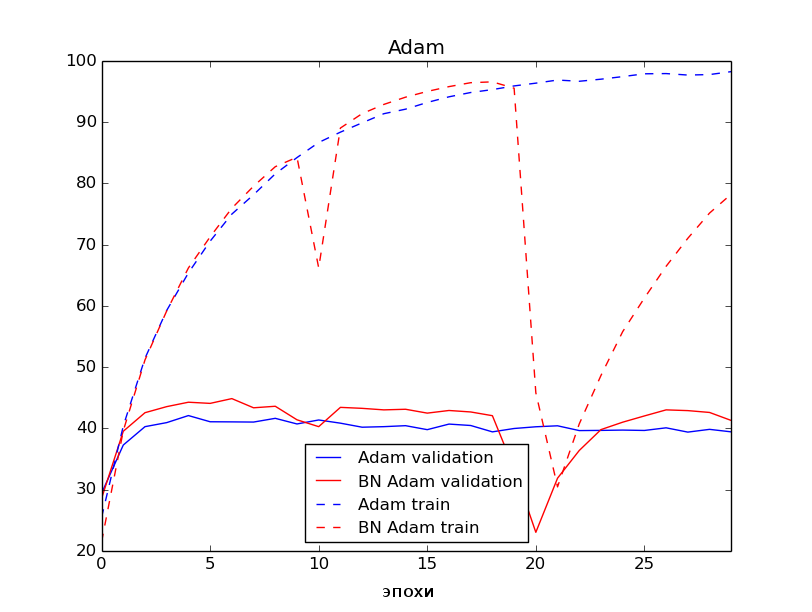
\includegraphics[scale=0.7]{adam_shallow.png}
\caption{\small Прыжки метода Adam при добавлении батч-нормализации} \label{fig:adam}
\end{figure}

Проблему окончательно изучить не удалось, однако на основе проведенных экспериментов удалось вывести несколько рекомендаций по использованию батч-нормализации.

%Теперь просто посмотрим на качество методов для глубоких сетей . Видно, что на первых эпохах методы 
%
%\begin{table}[h!]
%\centering
%\begin{tabular}{|c|c|c|c|c|c|}\hline
%Номер эпохи & 2 & 3 & 10 & 25 & 50 \\\hline\hline
%SGD & 10.64 & 10.64 & 19.65 & 47.38 & 90.55 \\\hline
%
%SGDm & 20.0 & 33.78 & 91.54 & 95.29 & 96.19 \\\hline
%
%Adam & 68.01 & 81.55 & 91.83 & 95.02 & 95.86 \\\hline
%
%Adagrad & 39.39 & 53.41 & 91.85 & 94.06 & 94.69 \\\hline
%
%Adadelta & 41.63 & 61.98 & 93.58 & 95.83 & 96.16 \\\hline
%
%RMSprop & 48.66 & 65.59 & 92.09 & 95.36 & 95.85 \\\hline
%
%\end{tabular}
%\caption{Качество методов на MNIST, deep MLP. На первых эпохах низкое качество}
%\end{table}
%
%
%\begin{table}[h!]
%\centering
%\begin{tabular}{|c|c|c|c|c|c|}\hline
%Номер эпохи & 1 & 5 & 10 & 20 & 50 \\\hline\hline
%SGD & 9.67 & 9.43 & 10.33 & 10.33 & 48.46 \\\hline
%
%SGDm & 9.43 & 9.43 & 17.47 & 32.8 & 71.01 \\\hline
%
%Adam & 21.33 & 38.71 & 51.72 & 59.16 & 71.44 \\\hline
%
%Adagrad & 10.11 & 27.44 & 40.39 & 47.71 & 58.87 \\\hline
%
%Adadelta & 9.67 & 11.77 & 13.23 & 34.67 & 48.87 \\\hline
%
%RMSprop & 12.97 & 20.47 & 38.2 & 47.24 & 66.04 \\\hline
%
%\end{tabular}
%\caption{Качество на CIFAR-10, deep CNN. На первых эпохах низкое качество}
%\end{table}


\newpage
\section{Заключение}

Батч-нормализация является прорывной идеей в области обучения нейронных сетей. Однако она не всегда повышает качество работы рассмотренных методов. Были сформулированы некоторые рекомендации по ее применению:

\begin{itemize}
\item Для полносвязной неглубокой архитектуры сети батч-нормализацию стоит применять к более простым методам. Например, методы, использующие инерцию, такие как SGDm, Adam, Adadelta, покажут хорошее качество и без батч-нормализации. А с ней они работают дольше и могут показать качество хуже.
\item Для глубоких сетей всегда нужно использовать батч-нормализацию, так как иначе методы могут совсем не обучаться.
\item Если время или количество эпох ограничено и очень мало, то обязательно стоит добавить в сеть батч-нормализацию, так как она сильнее всего помогает именно на первых эпохах.
\item Для метода Adam с батч-нормализацией нужно быть аккуратным: чтобы не возникло проблем при обучении, требуется аккуратно подобрать параметры метода.
\end{itemize}


\newpage
\addcontentsline{toc}{section}{Список литературы}
\begin{thebibliography}{99}


\bibitem{BN}
Ioffe, Sergey, and Christian Szegedy. "Batch normalization: Accelerating deep network training by reducing internal covariate shift." arXiv preprint arXiv:1502.03167 (2015).

\bibitem{cov_shift}
Shimodaira, Hidetoshi. "Improving predictive inference under covariate shift by weighting the log-likelihood function." Journal of statistical planning and inference 90.2 (2000): 227-244.

\bibitem{momentum}
Sutskever, Ilya, et al. "On the importance of initialization and momentum in deep learning." Proceedings of the 30th international conference on machine learning (ICML-13). 2013.

\bibitem{adagrad}
Duchi, John, Elad Hazan, and Yoram Singer. "Adaptive subgradient methods for online learning and stochastic optimization." The Journal of Machine Learning Research 12 (2011): 2121-2159.

\bibitem{rmsprop}
Tieleman, Tijmen, and Geoffrey Hinton. "Lecture 6.5-rmsprop: Divide the gradient by a running average of its recent magnitude." COURSERA: Neural Networks for Machine Learning 4 (2012): 2.

\bibitem{adadelta}
Zeiler, Matthew D. "ADADELTA: an adaptive learning rate method." arXiv preprint arXiv:1212.5701 (2012).

\bibitem{adam}
Kingma, Diederik, and Jimmy Ba. "Adam: A method for stochastic optimization." arXiv preprint arXiv:1412.6980 (2014).

\bibitem{eff_backprop}
LeCun, Yann A., et al. "Efficient backprop." Neural networks: Tricks of the trade. Springer Berlin Heidelberg, 2012. 9-48.

\bibitem{speech_recognition}
Waibel, Alexander, et al. "Phoneme recognition using time-delay neural networks." Acoustics, Speech and Signal Processing, IEEE Transactions on 37.3 (1989): 328-339.

\bibitem{time_series}
Kolarik, Thomas, and Gottfried Rudorfer. "Time series forecasting using neural networks." ACM Sigapl Apl Quote Quad. Vol. 25. No. 1. ACM, 1994.

\bibitem{comp_vis}
Krizhevsky, Alex, Ilya Sutskever, and Geoffrey E. Hinton. "Imagenet classification with deep convolutional neural networks." Advances in neural information processing systems. 2012.

\bibitem{backprop}
Hecht-Nielsen, Robert. "Theory of the backpropagation neural network." Neural Networks, 1989. IJCNN., International Joint Conference on. IEEE, 1989.

\bibitem{sgd}
Amari, Shunichi. "A theory of adaptive pattern classifiers." Electronic Computers, IEEE Transactions on 3 (1967): 299-307.

\bibitem{clmnist}
Mnih, Volodymyr, Nicolas Heess, and Alex Graves. "Recurrent models of visual attention." Advances in Neural Information Processing Systems. 2014.

\end{thebibliography}


\newpage
\addcontentsline{toc}{section}{Приложение}
\section*{Приложение}



%\section*{*На защиту выносится}
%
%По результатам экспериментов я хочу сделать выводы (из которых потом вынесу обобщения на защиту):
%
%\begin{enumerate}
%\item Чем метод лучше работает, тем БН его слабее улучшает (по сути есть эксперименты)
%\item Методы с инерцией плохо улучшаются БН на MLP (по сути есть эксперименты)
%\item Методы типа Adam, Adadelta, RMSprop плохо улучшаются БН на CNN (по сути есть эксперименты)
%\item БН сильнее улучшает методы на глубокой архитектуре (!) (вообще не сделаны эксперименты!!!)
%\item БН плохо сочетается с Адамом, появляются скачки (частичные эксперименты от Кати. ОБДУМАТЬ и доделать!)
%\item Рекомендации по использованию БН (включает все выше перечисленное)
%\item Подтверждение выводов статьи, что можно использовать большие рейты, что ускоряет обучение.
%\end{enumerate}


\begin{table}[h!]
\centering
\begin{tabular}{|c|c|c|c|c|c|}\hline
\textbf{Номер эпохи} & \textbf{2} & \textbf{5} & \textbf{20} & \textbf{35} & \textbf{50} \\\hline\hline
SGD & 10.64 & 10.64 & 19.65 & 47.38 & 90.55 \\\hline
BN SGD & 85.64 & 91.27 & 95.44 & 96.55 & 97.14 \\\hline
Улучшение & 0.84 & 0.9 & 0.94 & 0.93 & 0.7 \\\hline\hline
SGDm & 20.0 & 33.78 & 91.54 & 95.29 & 96.19 \\\hline
BN SGDm & 83.79 & 88.86 & 94.22 & 96.2 & 96.32 \\\hline
Улучшение & 0.8 & 0.83 & 0.32 & 0.19 & 0.03 \\\hline\hline
Adam & 68.01 & 81.55 & 91.83 & 95.02 & 95.86 \\\hline
BN Adam & 91.12 & 93.65 & 96.57 & 97.01 & 97.03 \\\hline
Улучшение & 0.72 & 0.66 & 0.58 & 0.4 & 0.28 \\\hline\hline
Adagrad & 39.39 & 53.41 & 91.85 & 94.06 & 94.69 \\\hline
BN Adagrad & 90.72 & 92.73 & 95.48 & 96.26 & 96.63 \\\hline
Улучшение & 0.85 & 0.84 & 0.45 & 0.37 & 0.37 \\\hline\hline
Adadelta & 41.63 & 61.98 & 93.58 & 95.83 & 96.16 \\\hline
BN Adadelta & 75.59 & 88.06 & 95.32 & 96.56 & 96.71 \\\hline
Улучшение & 0.58 & 0.69 & 0.27 & 0.18 & 0.14 \\\hline\hline
RMSprop & 48.66 & 65.59 & 92.09 & 95.36 & 95.85 \\\hline
BN RMSprop & 85.86 & 93.67 & 95.67 & 97.15 & 97.37 \\\hline
Улучшение & 0.72 & 0.82 & 0.45 & 0.39 & 0.37 \\\hline
\end{tabular}
\caption{Качество на MNIST, DEEP MLP}
\end{table}


\begin{table}
\centering
\begin{tabular}{|c|c|c|c|c|c|}\hline
\textbf{Номер эпохи} & \textbf{2} & \textbf{5} & \textbf{20} & \textbf{35} & \textbf{50} \\\hline\hline
SGD & 9.67 & 9.43 & 10.33 & 10.33 & 48.46 \\\hline
BN SGD & 47.77 & 66.79 & 74.13 & 80.41 & 83.61 \\\hline
Улучшение & 0.42 & 0.63 & 0.71 & 0.78 & 0.68 \\\hline\hline
SGDm & 9.43 & 9.43 & 17.47 & 32.8 & 71.01 \\\hline
BN SGDm & 49.14 & 68.27 & 75.76 & 79.4 & 83.15 \\\hline
Улучшение & 0.44 & 0.65 & 0.71 & 0.69 & 0.42 \\\hline\hline
Adam & 21.33 & 38.71 & 51.72 & 59.16 & 71.44 \\\hline
BN Adam & 50.04 & 73.53 & 80.62 & 84.2 & 86.37 \\\hline
Улучшение & 0.36 & 0.57 & 0.6 & 0.61 & 0.52 \\\hline\hline
Adagrad & 10.11 & 27.44 & 40.39 & 47.71 & 58.87 \\\hline
BN Adagrad & 28.84 & 61.41 & 75.4 & 81.64 & 84.67 \\\hline
Улучшение & 0.21 & 0.47 & 0.59 & 0.65 & 0.63 \\\hline\hline
Adadelta & 9.67 & 11.77 & 13.23 & 34.67 & 48.87 \\\hline
BN Adadelta & 47.1 & 63.65 & 72.35 & 78.35 & 82.19 \\\hline
Улучшение & 0.41 & 0.59 & 0.68 & 0.67 & 0.65 \\\hline\hline
RMSprop & 12.97 & 20.47 & 38.2 & 47.24 & 66.04 \\\hline
BN RMSprop & 23.97 & 59.22 & 77.36 & 82.63 & 86.79 \\\hline
Улучшение & 0.13 & 0.49 & 0.63 & 0.67 & 0.61 \\\hline
\end{tabular}
\caption{Качество на CIFAR-10, DEEP CNN}
\end{table}



%%%%%\begin{table}
%%%%%\centering
%%%%%\begin{tabular}{|c|c|c|c|c|c|}\hline
%%%%%Номер эпохи & 1 & 2 & 5 & 20 & 50 \\\hline
%%%%%SGD & 24.26 & 22.14 & 43.39 & 57.87 & 65.45 \\\hline
%%%%%BN SGD & 45.64 & 49.71 & 56.4 & 74.01 & 76.2 \\\hline
%%%%%Улучшение* & 0.28 & 0.35 & 0.23 & 0.38 & 0.31 \\\hline
%%%%%SGDm & 29.05 & 38.39 & 48.71 & 61.73 & 70.51 \\\hline
%%%%%BN SGDm & 53.72 & 58.76 & 67.96 & 75.26 & 78.39 \\\hline
%%%%%Улучшение* & 0.35 & 0.33 & 0.38 & 0.35 & 0.27 \\\hline
%%%%%Adam & 43.28 & 47.3 & 55.44 & 66.1 & 72.54 \\\hline
%%%%%BN Adam & 51.42 & 57.19 & 69.57 & 76.23 & 77.39 \\\hline
%%%%%Улучшение* & 0.14 & 0.19 & 0.32 & 0.3 & 0.18 \\\hline
%%%%%Adagrad & 29.82 & 37.25 & 48.02 & 59.57 & 64.63 \\\hline
%%%%%BN Adagrad & 48.24 & 53.83 & 63.15 & 74.19 & 76.96 \\\hline
%%%%%Улучшение* & 0.26 & 0.26 & 0.29 & 0.36 & 0.35 \\\hline
%%%%%Adadelta & 31.31 & 32.96 & 48.0 & 67.15 & 70.81 \\\hline
%%%%%BN Adadelta & 49.62 & 55.96 & 61.25 & 74.99 & 77.2 \\\hline
%%%%%Улучшение* & 0.27 & 0.34 & 0.25 & 0.24 & 0.22 \\\hline
%%%%%RMSprop & 25.6 & 39.89 & 49.58 & 63.37 & 70.31 \\\hline
%%%%%BN RMSprop & 42.61 & 52.98 & 61.61 & 74.94 & 75.81 \\\hline
%%%%%Улучшение* & 0.23 & 0.22 & 0.24 & 0.32 & 0.19 \\\hline
%%%%%\end{tabular}
%%%%%\caption{Качество на , лучшие рейты}
%%%%%\end{table}


%\begin{table}
%\centering
%\scriptsize
%\begin{tabular}{|c|c|c|c|c|c|}\hline
%Номер эпохи & 1 & 3 & 15 & 35 & 50 \\\hline\hline
%\textbf{SGD} & 89.15 & 92.84 & 96.81 & 97.58 & 97.73 \\\hline
%BN SGD & 96.42 & 97.38 & 98.14 & 98.18 & 98.23 \\\hline
%{Улучшение} & 0.67 & 0.63 & 0.42 & 0.25 & 0.22 \\\hline\hline
%\textbf{SGDm} & 93.39 & 96.4 & 97.83 & 98.03 & 98.03 \\\hline
%BN SGDm & 96.49 & 97.62 & 98.11 & 97.87 & 98.12 \\\hline
%{Улучшение} & 0.47 & 0.34 &  \textbf{0.13} &  \textbf{-0.08} &  \textbf{0.05} \\\hline\hline
%\textbf{Adam} & 93.47 & 96.03 & 97.62 & 98.04 & 98.02 \\\hline
%BN Adam & 94.85 & 96.81 & 97.51 & 97.75 & 98.16 \\\hline
%{Улучшение} &  \textbf{0.21} &  \textbf{0.2} & \textbf{-0.05} & \textbf{-0.15} & \textbf{0.07} \\\hline\hline
%\textbf{Adagrad} & 93.92 & 96.1 & 97.37 & 97.55 & 97.64 \\\hline
%BN Adagrad & 96.01 & 97.16 & 97.81 & 97.84 & 97.97 \\\hline
%{Улучшение} & 0.34 & 0.27 & 0.17 & 0.12 & 0.14 \\\hline\hline
%\textbf{Adadelta} & 94.28 & 96.7 & 97.51 & 98.04 & 98.2 \\\hline
%BN Adadelta & 95.98 & 96.97 & 97.72 & 98.04 & 98.26 \\\hline
%{Улучшение} & \textbf{0.3} & \textbf{0.08} & \textbf{0.08} & \textbf{-0.0} & \textbf{0.03} \\\hline\hline
%\textbf{RMSprop} & 94.58 & 96.14 & 96.75 & 97.34 & 97.27 \\\hline
%BN RMSprop & 96.12 & 97.18 & 97.88 & 97.91 & 97.95 \\\hline
%{Улучшение} & \textbf{0.28} & \textbf{0.27} & 0.35 & 0.21 & 0.25 \\\hline
%\end{tabular}
%\caption{\scriptsize Качество на MNIST + MLP, топ-3 наименьшего улучшения}
%\end{table}



%\begin{table}
%\centering
%\begin{tabular}{|c|c|c|c|c|c|c|}\hline
%Номер эпохи & 2 & 3 & 5 & 20 & 49 \\\hline\hline
%SGD & 29.02 & 34.7 & 35.33 & 42.89 & 48.74 \\\hline
%BN SGD & 45.66 & 46.54 & 49.44 & 54.69 & 57.23 \\\hline
%Улучшение* & 0.23 & 0.18 & 0.22 & 0.21 & 0.17 \\\hline\hline
%SGDm & 34.84 & 38.98 & 40.49 & 47.66 & 51.71 \\\hline
%BN SGDm & 45.63 & 46.73 & 49.21 & 54.29 & 56.77 \\\hline
%Улучшение* & 0.17 & 0.13 & 0.15 & 0.13 & 0.1 \\\hline\hline
%Adam & 36.94 & 38.93 & 42.31 & 47.99 & 51.36 \\\hline
%BN Adam & 45.31 & 46.44 & 48.69 & 54.59 & 57.28 \\\hline
%Улучшение* & 0.13 & 0.12 & 0.11 & 0.13 & 0.12 \\\hline\hline
%Adagrad & 28.4 & 30.94 & 33.25 & 42.77 & 46.11 \\\hline
%BN Adagrad & 46.16 & 46.97 & 48.88 & 53.21 & 55.52 \\\hline
%Улучшение* & 0.25 & 0.23 & 0.23 & 0.18 & 0.17 \\\hline\hline
%Adadelta & 30.46 & 36.07 & 34.86 & 42.98 & 48.48 \\\hline
%BN Adadelta & 42.94 & 44.77 & 47.12 & 52.59 & 55.98 \\\hline
%Улучшение* & 0.18 & 0.14 & 0.19 & 0.17 & 0.15 \\\hline\hline
%RMSprop & 32.45 & 34.42 & 35.97 & 40.35 & 48.45 \\\hline
%BN RMSprop & 46.1 & 46.34 & 49.32 & 53.47 & 56.64 \\\hline
%Улучшение* & 0.2 & 0.18 & 0.21 & 0.22 & 0.16 \\\hline\hline
%\end{tabular}
%\caption{Качество на CIFAR-10, MLP, лучшие рейты}
%\end{table}



%\begin{table}
%\centering
%\begin{tabular}{|c|c|c|c|c|c|c|c|c|c|}\hline
%Номер эпохи & 2 & 5 & 8 & 15 & 20 & 35 & 50 \\\hline\hline
%SGD & 96.37 & 97.71 & 98.14 & 98.49 & 98.51 & 98.46 & 98.8 \\\hline
%BN SGD & 98.7 & 99.01 & 99.12 & 99.21 & 99.2 & 99.22 & 99.24 \\\hline
%Улучшение* & 0.64 & 0.57 & 0.53 & 0.48 & 0.46 & 0.49 & 0.37 \\\hline\hline
%SGDm & 95.89 & 97.75 & 98.12 & 98.42 & 98.43 & 98.77 & 98.82 \\\hline
%BN SGDm & 98.78 & 98.91 & 99.03 & 99.16 & 99.16 & 99.19 & 99.17 \\\hline
%Улучшение* & 0.7 & 0.52 & 0.48 & 0.47 & 0.46 & 0.34 & 0.3 \\\hline\hline
%Adam & 97.64 & 98.57 & 98.81 & 98.92 & 99.08 & 99.12 & 99.16 \\\hline
%BN Adam & 98.68 & 98.82 & 99.01 & 99.23 & 99.22 & 99.25 & 99.25 \\\hline
%Улучшение* & 0.44 & 0.17 & 0.17 & 0.29 & 0.15 & 0.15 & 0.11 \\\hline\hline
%Adagrad & 98.0 & 98.6 & 98.81 & 98.91 & 99.01 & 98.92 & 98.96 \\\hline
%BN Adagrad & 98.92 & 99.13 & 99.13 & 99.25 & 99.29 & 99.24 & 99.3 \\\hline
%Улучшение* & 0.46 & 0.38 & 0.27 & 0.31 & 0.28 & 0.3 & 0.33 \\\hline\hline
%Adadelta & 98.16 & 98.61 & 98.95 & 99.1 & 99.11 & 99.22 & 99.22 \\\hline
%BN Adadelta & 98.51 & 98.71 & 99.07 & 99.31 & 99.36 & 99.34 & 99.36 \\\hline
%Улучшение* & 0.19 & 0.07 & 0.11 & 0.23 & 0.28 & 0.15 & 0.18 \\\hline\hline
%RMSprop & 97.87 & 98.73 & 98.92 & 99.1 & 98.91 & 98.97 & 99.1 \\\hline
%BN RMSprop & 98.59 & 99.01 & 99.12 & 99.2 & 99.31 & 99.34 & 99.34 \\\hline
%Улучшение* & 0.34 & 0.22 & 0.19 & 0.11 & 0.37 & 0.36 & 0.27 \\\hline\hline
%\end{tabular}
%\caption{Качество на MNIST, CNN, лучшие рейты}
%\end{table}


\end{document}
